\documentclass[preprint,preprintnumbers,amsmath,amssymb]{revtex4}
\usepackage{tikz}
\usepackage{xcolor}

\begin{document}

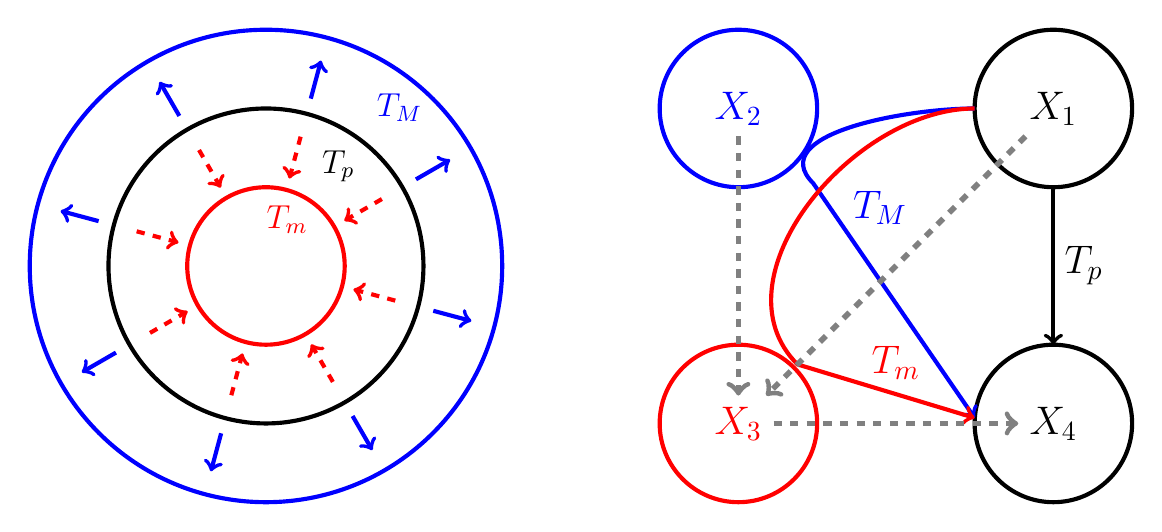
\begin{tikzpicture}[scale=1.0]

% Define circle radii
\def\innerRadius{1cm}
\def\middleRadius{2cm}
\def\outerRadius{3cm}
\def\smallRadius{1cm}

% Draw circles with thicker lines and larger font
\draw[red, line width=1.5pt] (0,0) circle (\innerRadius) node[above, font=\large] at (45:.38*\innerRadius) {$T_m$};
\draw[line width=1.5pt] (0,0) circle (\middleRadius) node[above, font=\large] at (45:.65*\middleRadius) {$T_p$};
\draw[blue, line width=1.5pt] (0,0) circle (\outerRadius) node[above, font=\large] at (45:.8*\outerRadius) {$T_M$};

% Draw red arrows from middle to inner circle with shorter length
\foreach \angle in {30,75,...,360}
  \draw[red, line width=1.5pt, dashed, ->] ({.85*\middleRadius*cos(\angle)}, {.85*\middleRadius*sin(\angle)}) -- ({1.15*\innerRadius*cos(\angle)}, {1.15*\innerRadius*sin(\angle)});

% Draw blue arrows from middle to outer circle with shorter length
\foreach \angle in {30,75,...,360}
  \draw[blue, line width=1.5pt, ->] ({1.1*\middleRadius*cos(\angle)}, {1.1*\middleRadius*sin(\angle)}) -- ({0.9*\outerRadius*cos(\angle)}, {0.9*\outerRadius*sin(\angle)});

% Panel with four smaller circles
\begin{scope}[shift={(8,0)}]

% Draw circles with labels
\draw[blue, line width=1.5pt] (-2,2) circle (\smallRadius) node[ font=\Large] (2) {$X_2$};
\draw[red, line width=1.5pt] (-2,-2) circle (\smallRadius) node [ font=\Large] (3) {$X_3$};
\draw[black, line width=1.5pt] (2,2) circle (\smallRadius) node [ font=\Large](1) {$X_1$};
\draw[black, line width=1.5pt] (2,-2) circle (\smallRadius) node [ font=\Large](4) {$X_4$};

% Arrows with labels
\draw[black, line width=1.5pt, ->] (2,1) -- (2,-1) node[midway, right, font=\Large] {$T_p$};
\draw[blue, line width=1.5pt, ->] (\smallRadius,2) to[out=180,in=135] (-1.05,1.05) -- (2-1,2-2*\smallRadius);
\draw[red, line width=1.5pt, ->] (\smallRadius,2) to[out=180,in=135] (-1.25,-1.25)  -- (2-1,2-2*\smallRadius);

% Dashed green arrows

\path [->,draw, dashed, color=gray, line width=2pt](1) edge node[left] {} (3);
\path [->,draw, dashed, color=gray, line width=2pt](2) edge node[left] {} (3);
\path [->,draw, dashed, color=gray, line width=2pt](3) edge node[left] {} (4);

\node[below, font=\Large, red] at (0,-.9) {$T_m$};

\node[above, font=\Large, blue] at (-.2,0.4) {$T_M$};


\end{scope}
\end{tikzpicture}

\end{document}